\documentclass{llncs}
\usepackage{times}
\usepackage[T1]{fontenc}

% Comentar para not MAC Users
%\usepackage[applemac]{inputenc}

\usepackage{a4}
%\usepackage[margin=3cm,nohead]{geometry}
\usepackage{epstopdf}
\usepackage{indentfirst}
\usepackage{graphicx}
\usepackage{float}
\usepackage{fancyvrb}
\usepackage{amsmath}
%\renewcommand{\baselinestretch}{1.5}

\begin{document}
\mainmatter
\title{TP3: Camada de Ligação Lógica: Ethernet e Protocolo ARP}

\titlerunning{TP3: Camada de Ligação Lógica: Ethernet e Protocolo ARP}

\author{Diogo Braga \and João Silva \and Ricardo Caçador}

\authorrunning{Diogo Braga \and João Silva \and Ricardo Caçador}

\institute{
University of Minho, Department of  Informatics, 4710-057 Braga, Portugal\\
e-mail: \{a82547,a82005,a81064\}@alunos.uminho.pt\\
PL4, Grupo 7
}

\date{}
\bibliographystyle{splncs}

\maketitle

\section{Captura e análise de Tramas Ethernet}

\subsection{Exercício 1}
\emph{Anote os endereços MAC de origem e de destino da trama capturada.}

\begin{figure}[H]
\begin{center}
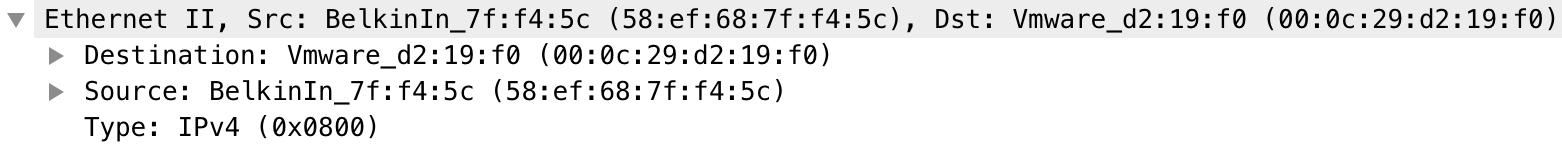
\includegraphics[scale=0.45]{1.png} 
\end{center}
\caption{\label{fig:1}Ethernet II}
\end{figure} 
\par
\textbf{R:} Como se pode observar na figura \ref{fig:1}, o endereço MAC de origem da trama
capturada é \textbf{58:ef:68:7f:f4:5c}, enquanto o endereço de destino é 
\textbf{00:0c:29:d2:19:f0}.


\subsection{Exercício 2}
\emph{Identifique a que sistemas se referem. Justifique.}
\\ \par
\textbf{R:} Como se pode observar na figura \ref{fig:1}, o endereço de origem refere-se à
interface de comunicação da nossa máquina. Neste caso, estamos conectados com um adaptador
\emph{belkin}, daí a parte do endereço
de origem atribuída ao fabricante estar assim designada. O endereço de destino refere-se
ao router de acesso da nossa rede local. Neste caso, o fabricante é a \emph{Vmware}.


\subsection{Exercício 3}
\emph{Qual o valor hexadecimal do campo Type da trama Ethernet? O que significa?}
\\ \par
\textbf{R:} Como se pode observar na figura \ref{fig:1}, o valor é \textbf{0x0800}.
Este campo é usado para indicar o protocolo que é encapsulado no payload do frame, sendo
que neste caso é o \textbf{IPv4}.


\subsection{Exercício 4}
\emph{Quantos bytes são usados desde o início da trama até ao caracter ASCII "G" do
método HTTP GET? Calcule e indique, em percentagem, a sobrecarga (overhead) introduzida
pela pilha protocolar no envio do HTTP GET.}

\begin{figure}[H]
\begin{center}
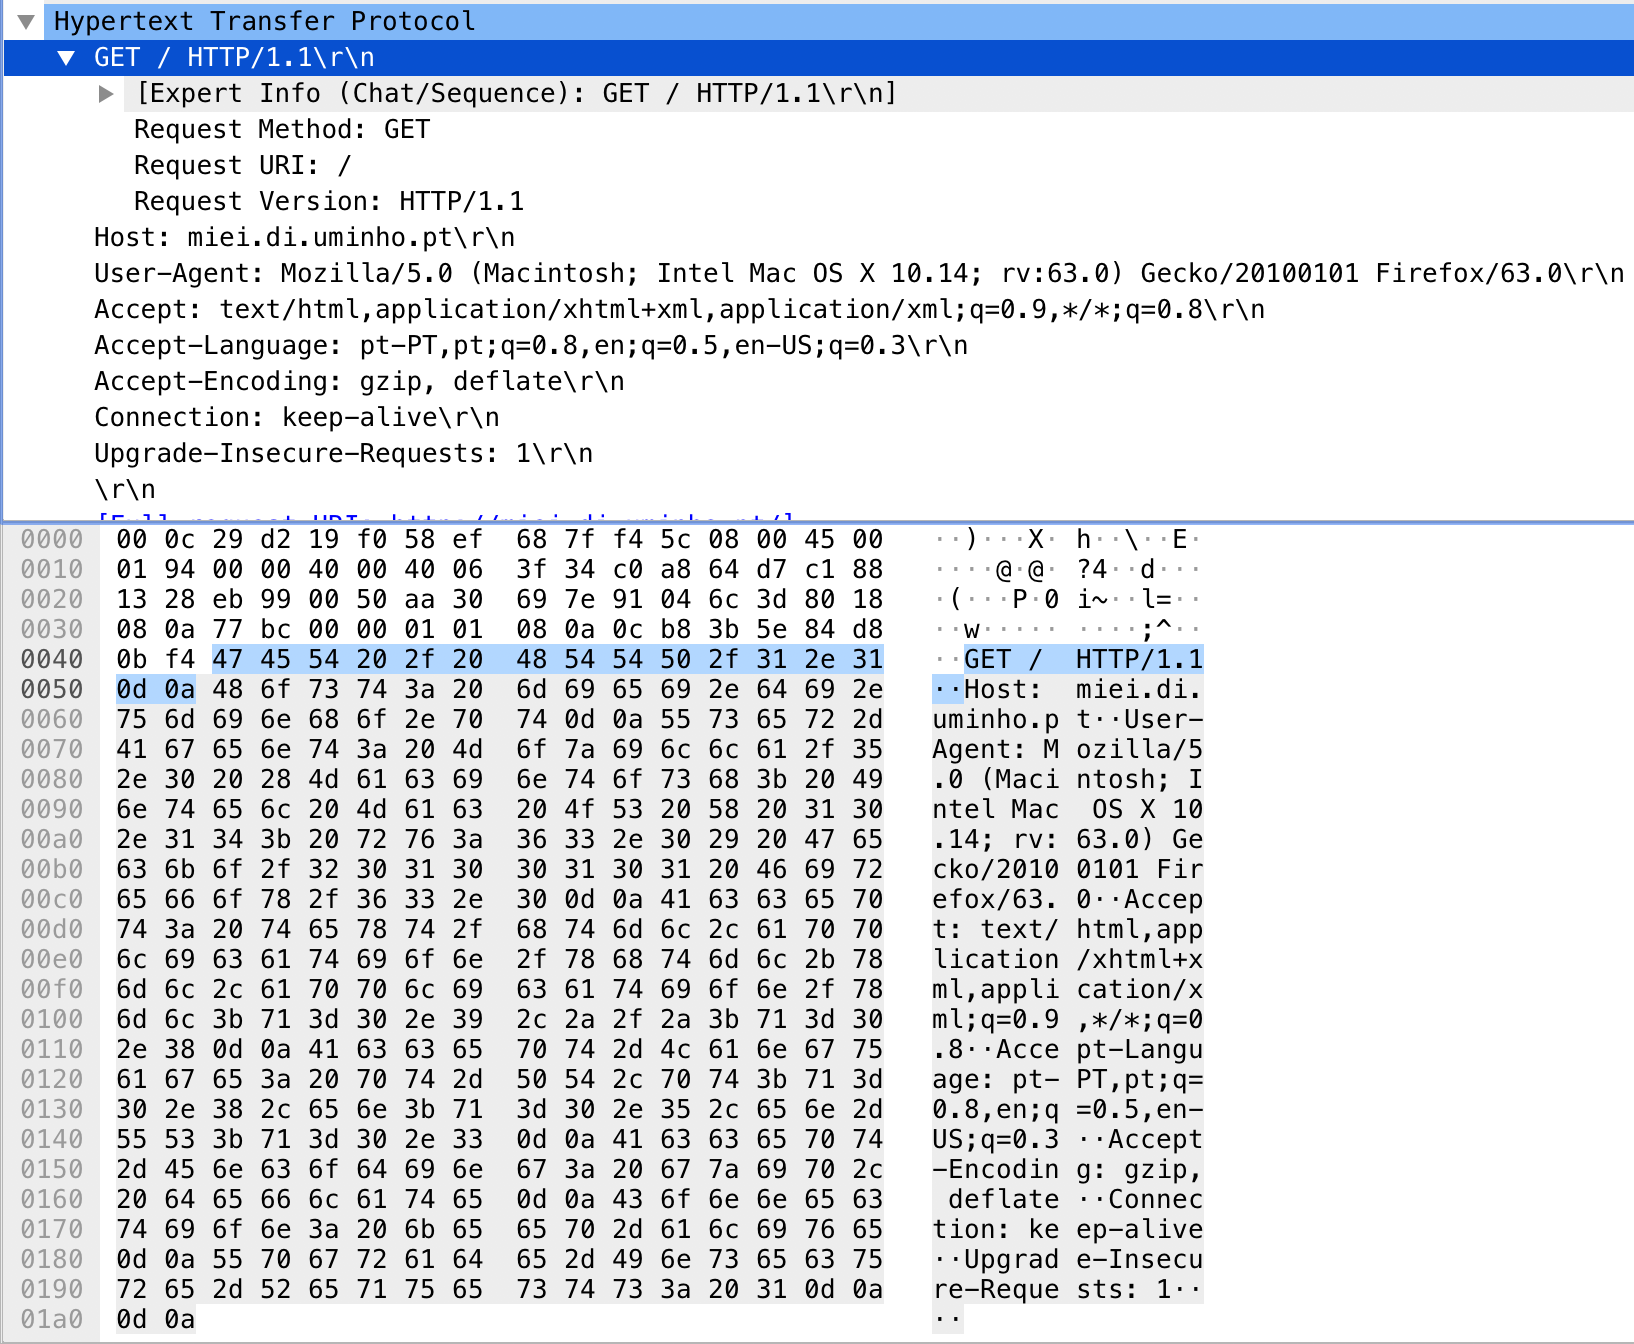
\includegraphics[scale=0.45]{4.png} 
\end{center}
\caption{\label{fig:4}HTTP GET}
\end{figure} 
\par
\textbf{R:} Até ao caracter ASCII "G" são usados \textbf{66 bytes}, enquanto no total são
usados \textbf{418 bytes}. Deste modo, o overhead introduzido pela pilha protocolar é
calculado divindindo 66 por 418, e multiplicando por 100, resulta em \textbf{15.79\%}. Tal
pode ser verificado na figura \ref{fig:4}.


\subsection{Exercício 5}
\emph{Através de visualização direta de uma trama capturada, verifique que, possivelmente,
o campo FCS (Frame Check Sequence) usado para deteção de erros não está a ser usado. Em 
sua opinião, porque será?}
\\ \par
\textbf{R:} Como estamos perante uma ligação Ethernet, e como este tipo de ligação
especifica que uma trama danificada deve ser descartada, não é necessário que exista
o campo FCS, uma vez que este género de ligação não especifica nenhuma ação que faça com
que a trama seja retransmitida. Neste caso a ocorrência de erros é ínfima, mas por 
exemplo, no caso da ligação Wireless o campo FCS certamente estaria presente na 
trama, visto este tipo de ligação ser mais sucestível a ruído e erros.


\subsection{Exercício 6}
\emph{Qual é o endereço Ethernet da fonte? A que sistema de rede corresponde? Justifique.}
\\ \par
\textbf{R:} O endereço da fonte é \textbf{00:0c:29:d2:19:f0}, que corresponde ao router
da rede local. Uma vez que recebemos a resposta do endereço da interface IP 193.136.19.40,
a nível de ligação de dados o router tem uma tabela que permite fazer o mapeamento entre
endereços de nível de rede e endereços de nível de ligação lógica. Como o nível de ligação
lógica apenas conhece os hosts da rede local, a trama é entregue no destino 
58:ef:68:7f:f4:5c, que corresponde ao endereço de IP 192.168.100.215.


\subsection{Exercício 7}
\emph{Qual é o endereço MAC do destino? A que sistema corresponde?}
\\ \par
\textbf{R:} O endereço de destino é \textbf{58:ef:68:7f:f4:5c}, e corresponde à interface
de comunicação do nosso computador.


\subsection{Exercício 8}
\emph{Atendendo ao conceito de desencapsulamento protocolar, identifique os vários 
protocolos contidos na trama recebida.}
\\ \par
\textbf{R:} Os protocolos contidos na trama recebida são o HTTP a nível aplicacional, o
TCP a nível de transporte e o IPv4 a nível de rede.


\section{Protocolo ARP}

\subsection{Exercício 9}
\emph{Observe o conteúdo da tabela ARP. Diga o que significa cada uma das colunas}

\begin{figure}[H]
\begin{center}
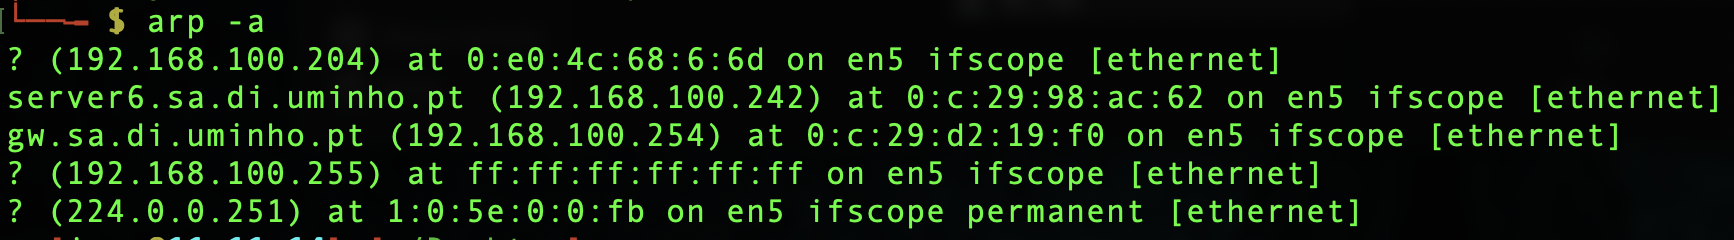
\includegraphics[scale=0.45]{9.png} 
\end{center}
\caption{\label{fig:9}Tabela ARP}
\end{figure} 
\par
\textbf{R:} As tabelas ARP fazem o mapeamento entre endereços de rede e endereços de nível de ligação de dados. Como se pode observar na figura \ref{fig:9}, a primeira coluna da tabela corresponde aos endereços de nível 3, enquanto a segunda coluna corresponde aos endereços de nível 2.


\subsection{Exercício 10}
\emph{Qual é o valor hexadecimal dos endereços de origem e destino na trama Ethernet
que contém a mensagem com pedido ARP (ARP Request)? Como interpreta e justifica o 
endereço destino usado?}

\begin{figure}[H]
\begin{center}
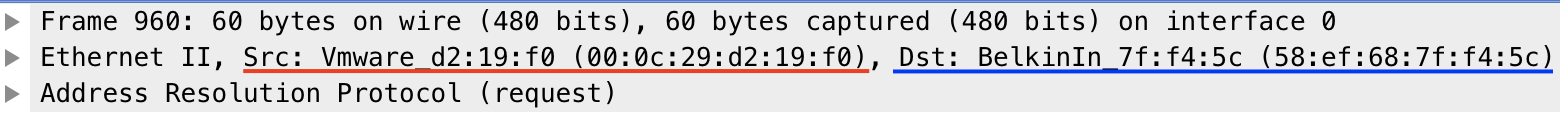
\includegraphics[scale=0.45]{10.png} 
\end{center}
\caption{\label{fig:10}Origem e Destino da Trama Ethernet}
\end{figure} 
\par
\textbf{R:} O endereço de origem da trama Ethernet encontra-se sublinhado a vermelho na figura \ref{fig:10}, cujo valor é \textbf{00:0c:29:d2:19:f0}. Por outro lado, o endereço de destino é \textbf{58:ef:68:7f:f4:5c}, e encontra-se sublinhado a azul na mesma figura. O endereço de destino identifica o nosso computador, tal é conclusível porque estamos perante uma situação em que o router tenta ter conexão a nível de ligação de dados com este mesmo, visto já saber o seu endereço IP.


\subsection{Exercício 11}
\emph{Qual o valor hexadecimal do campo tipo da trama Ethernet? O que indica?}

\begin{figure}[H]
\begin{center}
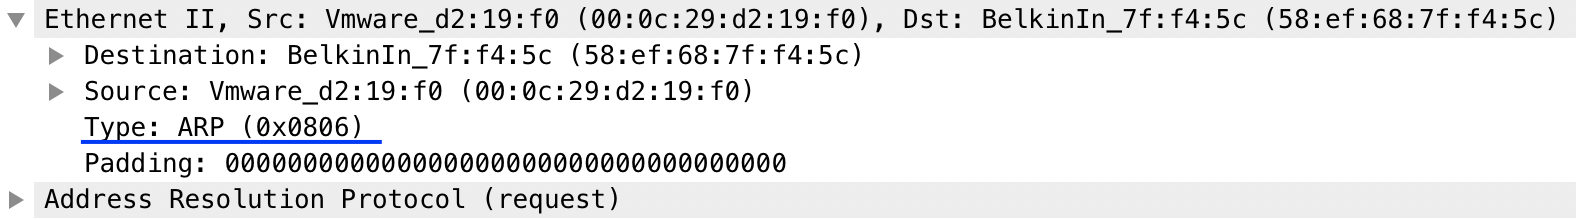
\includegraphics[scale=0.45]{11.png} 
\end{center}
\caption{\label{fig:11}Tipo da Trama Ethernet}
\end{figure} 
\par
\textbf{R:} Como se pode visualizar na figura \ref{fig:11} sublinhado a azul, o valor do campo tipo é \textbf{0x0806}, e indica o protocolo que vai encapsulado dentro da trama Ethernet, neste caso ARP.


\subsection{Exercício 12}
\emph{Qual o valor do campo ARP opcode? O que especifica? Se necessário, consulte a
RFC do protocolo ARP http://tools.ietf.org/html/rfc826.html.}

\begin{figure}[H]
\begin{center}
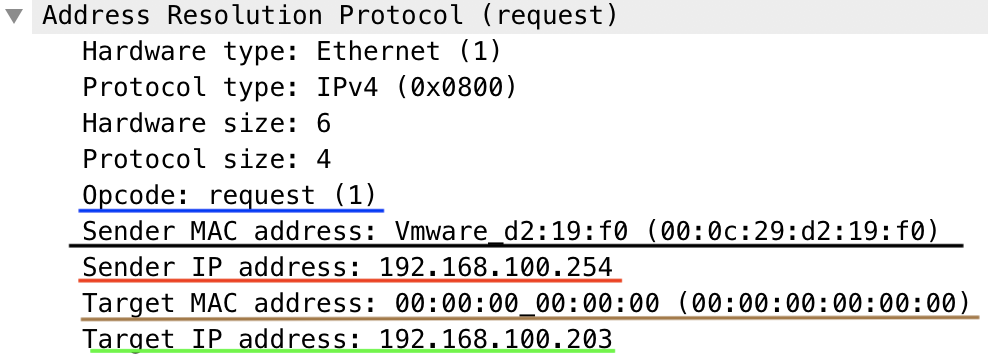
\includegraphics[scale=0.45]{12_13.png} 
\end{center}
\caption{\label{fig:12_13}ARP Request}
\end{figure} 
\par
\textbf{R:} O valor do campo ARP opcode é \textbf{request (1)}, tal como pode ser verificável na figura \ref{fig:12_13} sublinhado a azul. O opcode serve para determinar se a mensagem ARP é um pedido ou uma resposta ao pedido anterior. 


\subsection{Exercício 13}
\emph{Identifique que tipo de endereços estão contidos na mensagem ARP? Que conclui?}
\\ \par
\textbf{R:} Existem dois endereços do tipo MAC Adress e dois do tipo IP. A nível de rede, sabemos que o endereço de origem, sublinhado a vermelho, pretende comunicar com o endereço destino, sublinhado a verde. A nível de ligação de dados, conhecemos o endereço de origem sublinhado a preto, mas não temos conhecimento de qual seja o endereço de destino, pelo que enviamos para o endereço broadcast, sublinhado a castanho. Tal pode ser também verificável na figura \ref{fig:12_13}.


\subsection{Exercício 14}
\emph{Explicite que tipo de pedido ou pergunta é feita pelo host de origem?}

\begin{figure}[H]
\begin{center}
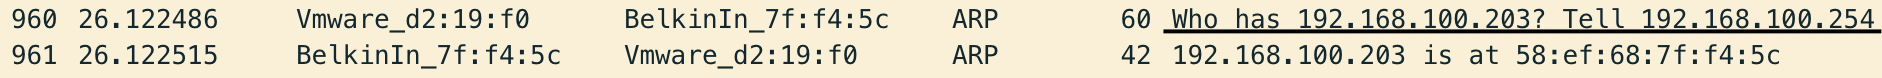
\includegraphics[scale=0.45]{14.png} 
\end{center}
\caption{\label{fig:14}Request ARP}
\end{figure} 
\par
\textbf{R:} Como se pode visualizar na figura \ref{fig:14} sublinhado a preto, o host de origem pergunta quem tem o endereço 192.168.100.203, e diz para o tal o comunicar ao endereço 192.168.100.254.


\subsection{Exercício 15}
\emph{Localize a mensagem ARP que é a resposta ao pedido ARP efectuado.}

\subsubsection{a.}
\emph{Qual o valor do campo ARP opcode? O que especifica?}

\begin{figure}[H]
\begin{center}
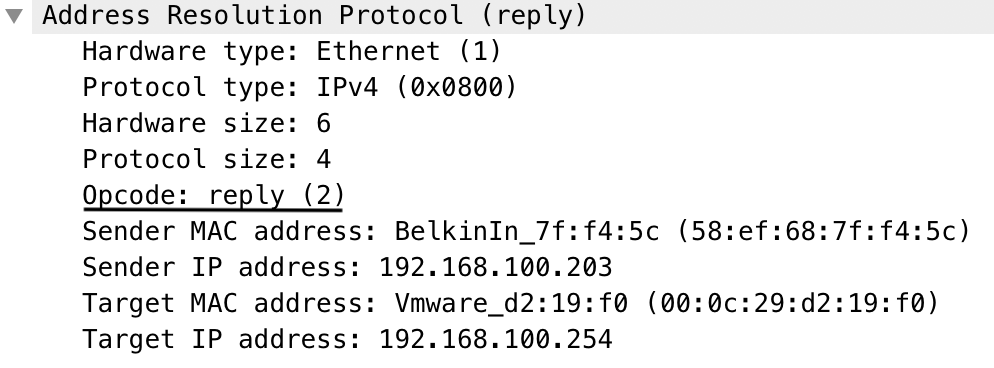
\includegraphics[scale=0.45]{15_a.png} 
\end{center}
\caption{\label{fig:15_a}ARP Reply}
\end{figure} 
\par
\textbf{R:} Como se pode visualizar na figura \ref{fig:15_a} sublinhado a preto, o valor do campo ARP opcode é \textbf{reply (2)}. Uma vez que o endereço do destino do pedido é igual ao endereço do nosso computador, este envia um ARP Reply.


\subsubsection{b.}
\emph{Em que posição da mensagem ARP está a resposta ao pedido ARP?}
\\ \par
\textbf{R:} A resposta ao pedido ARP encontra-se no campo \textbf{Sender MAC address}, uma vez que este tem o endereço que o router procura, e portanto responde ao request.

\newpage

\section{ARP Gratuito}

\subsection{Exercício 16}
\emph{Identifique um pacote de pedido ARP gratuito originado pelo seu sistema. Analise o 
conteúdo de um pedido ARP gratuito e identifique em que se distingue dos restantes
pedidos ARP. Registe a trama Ethernet correspondente. Qual o resultado esperado face ao
pedido ARP gratuito enviado?}

\begin{figure}[H]
\begin{center}
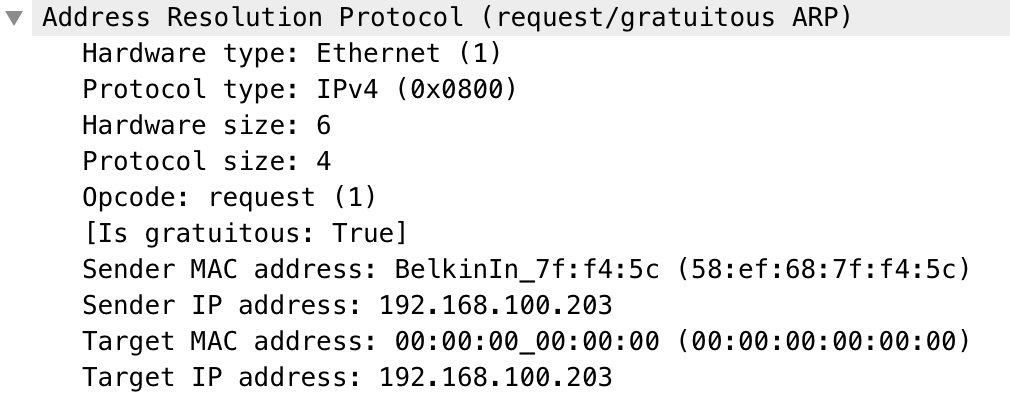
\includegraphics[scale=0.45]{16_gratuito.png} 
\end{center}
\caption{\label{fig:16_gratuito}ARP Request Gratuito}
\end{figure} 
\par
\begin{figure}[H]
\begin{center}
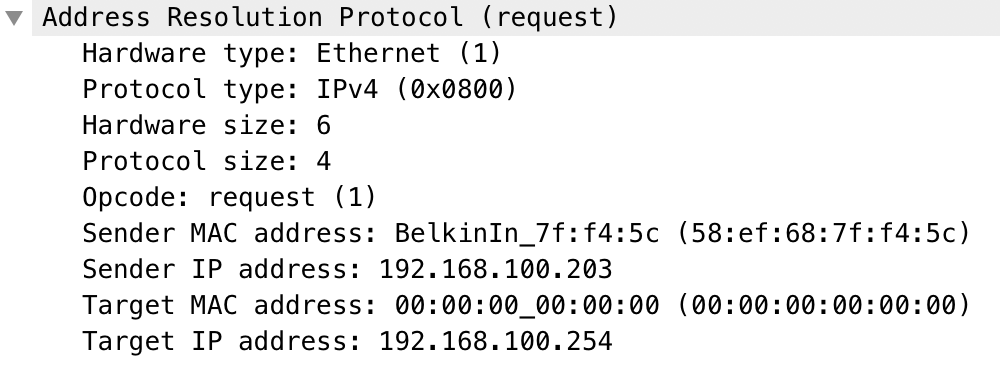
\includegraphics[scale=0.45]{16_request_normal.png} 
\end{center}
\caption{\label{fig:16_request_normal}ARP Request Normal}
\end{figure} 
\par
\textbf{R:} Como pode ser verificado nas figuras \ref{fig:16_gratuito} e 
\ref{fig:16_request_normal}, os endereços IP origem e destino do ARP Request gratuito são iguais, algo que não se verifica nos ARP Request normais. Isto porque nos ARP Request normais pretende-se saber qual o MAC Adress de um determinado endereço IP. Por outro lado, no ARP Request gratuito pretende-se anunciar um endereço MAC para que todos os sistemas na rede local possam atualizar as suas tabelas ARP.


\section{Domínios de colisão}

\begin{figure}[H]
\begin{center}
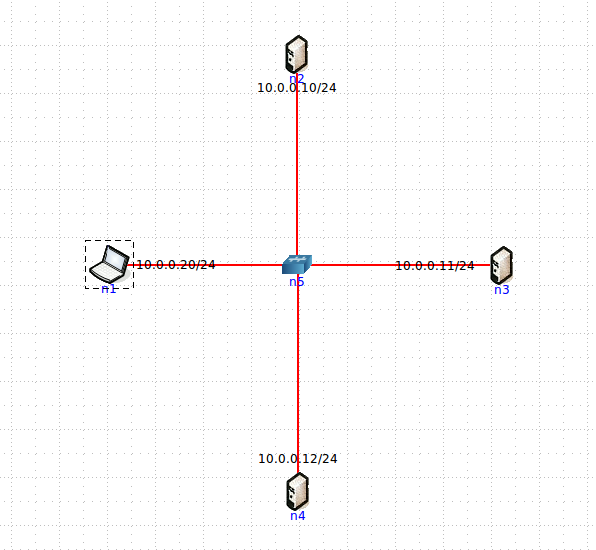
\includegraphics[scale=0.45]{17_topologia.png} 
\end{center}
\caption{\label{fig:17_topologia}Topologia com Hub}
\end{figure} 
\par

\begin{figure}[H]
\begin{center}
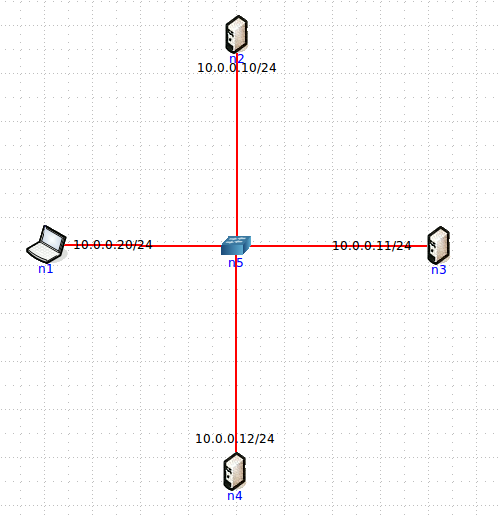
\includegraphics[scale=0.45]{18_topologia.png} 
\end{center}
\caption{\label{fig:18_topologia}Topologia com Switch}
\end{figure} 
\par


\subsection{Exercício 17}
\emph{Faça ping de n1 para n2. Verifique com a opção tcpdump como flui o tráfego
nas diversas interfaces dos vários dispositivos. Que conclui?}

\begin{figure}[H]
\begin{center}
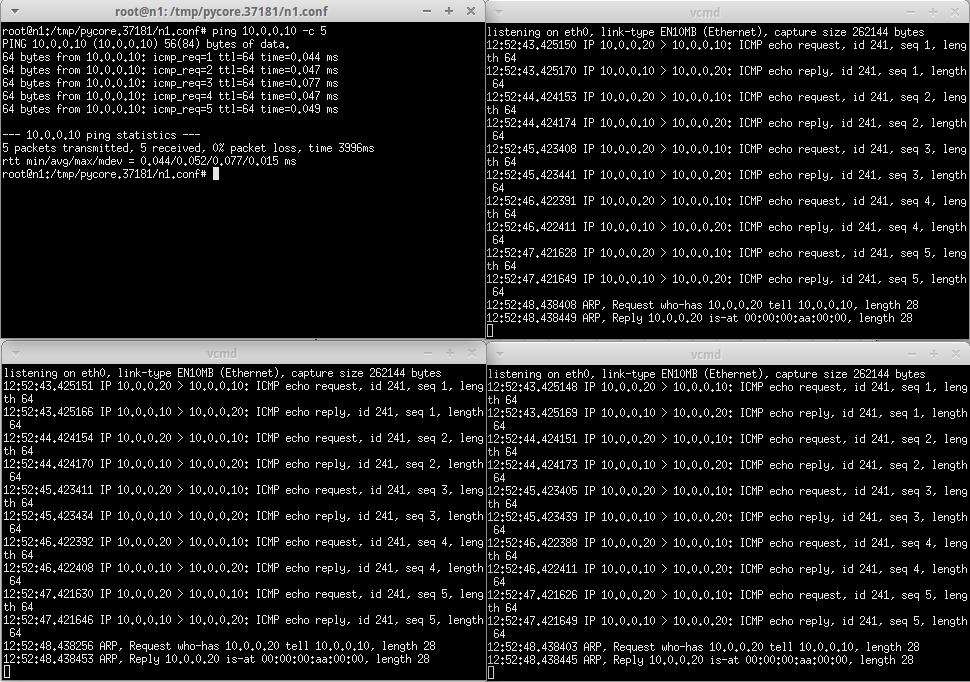
\includegraphics[scale=0.45]{17_fluxo.png} 
\end{center}
\caption{\label{fig:17_fluxo}Fluxo com Hub}
\end{figure} 
\par
\textbf{R:} Como pode ser verificado na figura \ref{fig:17_fluxo}, usando um Hub e executando o campo ping a partir do laptop n1, o Hub replica o fluxo para todos os servidores, tal é possível ver na figura uma vez que utilizamos o tcpdump em cada servidor para verificar o fluxo de tráfego. Um Hub é por consequência mais suscetível a ocorrência de colisões.


\subsection{Exercício 18}
\emph{Na topologia de rede substitua o hub por um switch. Repita os procedimentos que
realizou na pergunta anterior. Comente os resultados obtidos quanto à utilização de 
hubs e switches no contexto de controlar ou dividir domínios de colisão. Documente as
suas observações e conclusões com base no tráfego observado/capturado.}

\begin{figure}[H]
\begin{center}
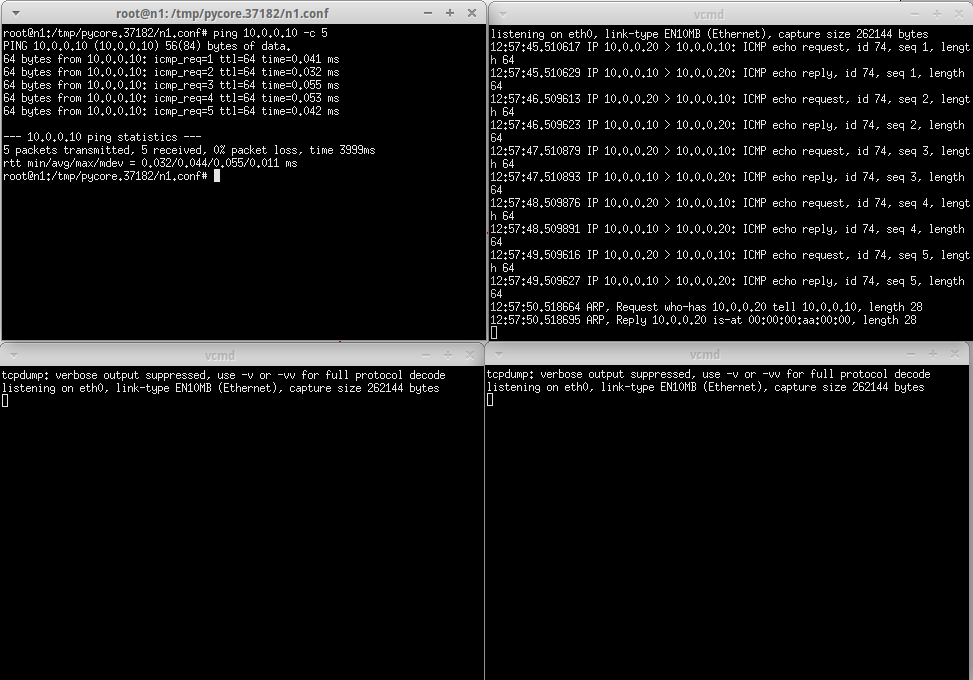
\includegraphics[scale=0.45]{18_fluxo.png} 
\end{center}
\caption{\label{fig:18_fluxo}Fluxo com Switch}
\end{figure} 
\par
\textbf{R:} Como pode ser verificado na figura \ref{fig:18_fluxo}, usando um Switch e executando o campo ping a partir do laptop n1, o Switch tem capacidade para enviar o fluxo só para o servidor pretendido, diminuindo assim a ocorrência de colisões, ao contrário dum Hub. Na figura, com auxílio do tcpdump aberto em cada servidor, é possível verificar tal ocorrência.


\section{Conclusão}
Neste trabalho prático dividido em 4 partes, abordamos principalmente temas como a Ethernet e o Protocolo ARP.

Na primeira secção trabalhamos com tramas Ethernet, e analisamos a fundo a questão dos endereços de nível lógico, também conhecidos com \textbf{MAC Address}

Na segunda secção abordamos o protocolo ARP, que inclui a análise de tabelas ARP presentes tanto nos end-systems como nos routers da rede local. Aprendemos também de uma forma muito prático como é feita a comunicação entre o router e um end-system a nível de ligação de dados.

Na terceira secção abordamos a questão do ARP gratuito, e foi de facto interessante perceber que quando um novo host entra numa rede local envia uma mensagem ARP a todos os hosts, para que estes possam atualizar as suas tabelas.

Na quarta e última secção tratamos da questão dos domínios de colisões, onde pusemos lado a lado um Hub e um Switch de forma a comparar o seu funcionamento e questões relacionadas com colisões na transmissão de tramas Ethernet.

Concluindo, com este guião exploramos a fundo as questões do nível de ligação de dados, e conseguimos de forma muito prática aprender os conceitos mais teóricos do funcionamento dos mecanismos desta camada.

\end{document}